\documentclass[11pt,english]{AMdocument}
\usepackage[utf8]{inputenc}
\usepackage{csquotes}
\usepackage{graphicx}
\usepackage{caption}
\usepackage{siunitx}
\usepackage{enumerate}

\AMsetColor{section=black,url=TUMGreen,link=TUMOrange,caption label=TUMGreen}

\title{Scenario \enquote{Hardening Shift Forks}}
\subtitle{Automated Hardening Process of Shift Forks at ZF Friedrichshafen}

\begin{document}
	\maketitle
	
	\section*{Executive Summary}

The scenario \enquote{Hardening Shift Forks} shall be automated using a mobile manipulator platform. It consists of a typical pick-and-place task including object recognition, motion planning, navigation as well as safe interaction with human co-workers. The task can be summarized as follows:

\begin{enumerate}
	\item A movable container has to be moved to the hardening machine.
	\item In a second, step shift forks have to be picked up from the container and positioned in the hardening machine.
	After the hardening process is finished, the shift fork has to be removed from the hardening machine and be put to
	another container. 
	\item Filled containers have to be moved to another waiting area.
	\item Random samples of hardened shift forks have to be transported to an inspection unit of a human worker.
\end{enumerate}

	\section*{Detailed Description}

The proposed scenario is related to the hardening process of shift forks at ZF Friedrichshafen AG. It can be summarized in four production steps as depicted in \cref{fig:img1}: 

\begin{figure}[ht]
	\centering
	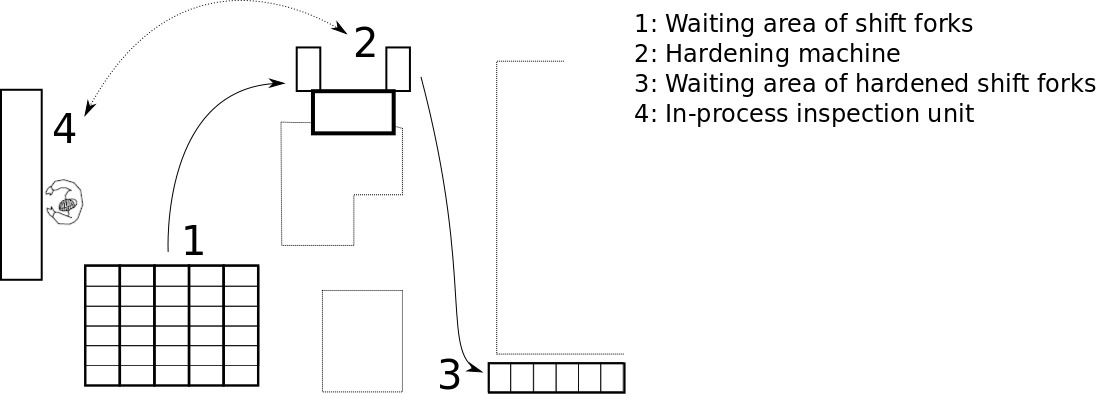
\includegraphics[width=0.8\textwidth]{img001}
	\caption{Floor plan indicating the working positions in setup of use-case.}
	\label{fig:img1}
\end{figure}

		\subsection*{Step 1}

Five different types of shift forks with an approximate weight of \SI{4}{kg} and a size of \num{0.3 x 0.1 x 0.03}\si{m} are provided by an employee at a predefined place. Its location is marked as 1. The shift forks are stored in containers in an arbitrary arrangement. Respectively four containers are stacked on top of each other on a wagon. The wagons are lined up side by side according to the type of fork in five lines as depicted in \cref{fig:img1} (see also \cref{fig:img3}). In step 1, the wagons have to be moved successively to the hardening machine (marked as 2 in \cref{fig:img1}). The hardening machine is equipped with a frame corresponding to the current type of shift fork. 

		\subsection*{Step 2}

Thus, in step 2, shift forks have to be picked from the container and placed into the frame of the hardening machine (see \cref{fig:img2}). Then the machine has to be started.

\begin{figure}[h]
	\centering
	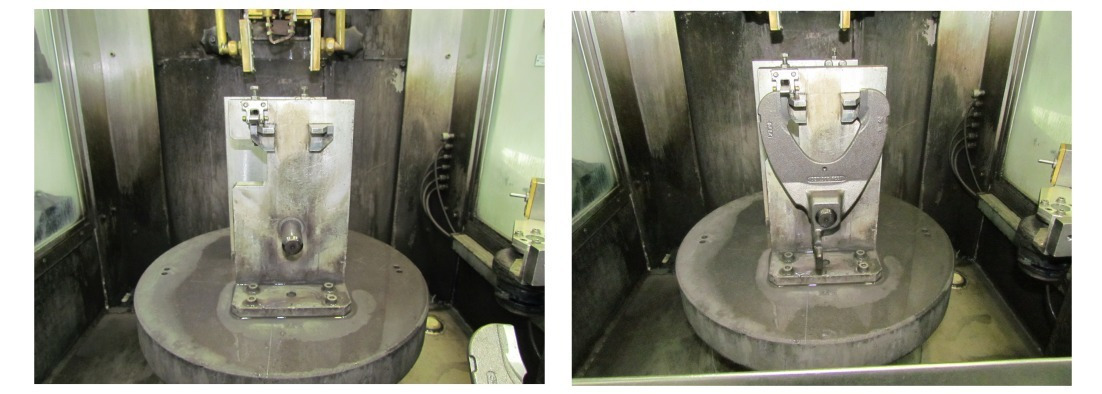
\includegraphics[width=\textwidth]{img002}
	\caption{Hardening machine with the frame (left) and a shift fork in the frame (right).}
	\label{fig:img2}
\end{figure}

		\subsection*{Step 3}

After the hardening process the current shift fork has to be removed from the hardening machine and be placed in an arbitrary arrangement in a different container. In step 3 the wagon with the stacked containers filled with hardened shift forks has to be moved to a defined end position (marked as 3 in \cref{fig:img1}) where an employee moves them to the next production step.

		\subsection*{Step 4}

After a certain number of forks (approx. 100) are treated, the hardening process has to be interrupted for quality control. For this reason the currently processed shift fork has to be taken to the inspection unit and handed over to a human employee who performs the inspection on the part (step 4, see \cref{fig:img1}). In \cref{fig:img3} the real setup of the first two working positions at ZF Friedrichshafen AG is shown. Hence, our objective is to establish the hardware platform used in this challenge for production steps 1-3. The in-process inspection is still performed by a human employee due to its complexity (visual inspection, hardness test) and the necessary expert evaluation by a skilled human worker. It could be automatized in the future.  

\begin{figure}[h]
	\centering
	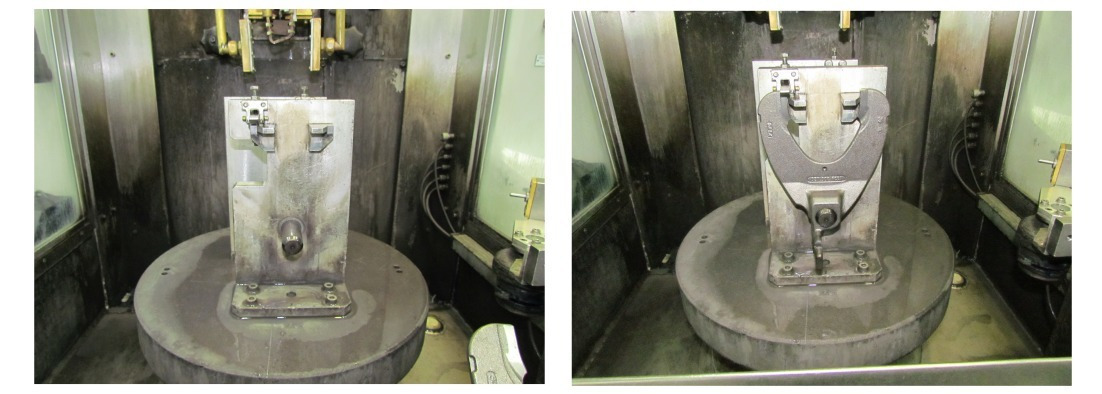
\includegraphics[width=\textwidth]{img003}
	\caption{Real setup in plant at ZF Friedrichshafen AG. Pictures are numbered according to working positions in hardening process (compare \cref{fig:img1}).}
	\label{fig:img3}
\end{figure}


	\section*{Simplified Scenario}

Single subtasks can be tested separately in the lab in order to facilitate the initial phase of the project:

\begin{enumerate}[I]
	\item Autonomous navigation of the platform with avoidance of obstacles and people.
	\item Moving the wagon with the containers.
	\item Picking and placing of the shift forks in the hardening machine.
\end{enumerate}

For task I., a simplified plant will be simulated, with fixed walls (or big boxes) and random positioning of obstacles and moving people. The platform will have to navigate between known positions, avoiding walls, obstacles and people on the way.

For task II., we will place one wagon at an arbitrary location in a given area. The robot will have to identify it and move it to a second (precisely specified) location along an unobstructed floor.

For testing task III. we will use 2 different types of shift forks in two separate containers. For each, we will have an example of the corresponding hardening machine frame. The platform will be on a fixed spot, as well as the container and its corresponding frame, in positions similar to the use case (see Position 2 in \cref{fig:img1}). The robot will have to identify the container’s type, locate one part, pick it and place it in the frame. Finally, it will have to remove it from the frame and place it again in the container. Here a strategy to manage the container placements around the machine will be defined.


	\section*{Main Aspects}

\begin{itemize}
	\item Autonomous navigation in a dynamically changing environment. The platform has to share its workspace with several co-workers and different types of obstacles can change their location over time.
	\item Safe interaction with human co-workers. This is especially true for step 4, where a human operator needs to be on the scene to perform the inspection of the parts.
	\item Intuitive human robot communication for efficient interaction and collaboration with operator. 
	\item Minimization of changeover times: changing the type series can be triggered by a superordinate production plan or the human operator. The high-level control framework for the upcoming task is set-up automatically while it supports the operator in choosing the appropriate end-effector for the robot system and changeover task for the hardening machine.
	\item Precise and reliable object recognition and handling. The shift forks are in the containers in arbitrary locations and have to be placed precisely into the frame.
	\item Intelligent high-level control system. The control system has to assess and react to varying conditions and tasks. The unit number for parts of the same type is small and vary depending on the order-book. This has to be treated together with varying environment conditions.
	\item Exploitation of force-torque sensing for external parameters identification (e.g. exact gripped object pose and properties, external loads, collision detection).
\end{itemize}


\end{document}
